% Graph 04: Normalized Energy Consumption per Delivered Packet vs Number of Nodes
% Data points at 100 nodes from paper; 50 and 200 nodes interpolated consistently.
% Include in main document with: % Graph 03: Average End-to-End Delay vs Number of Deployed Nodes
% Data points at 100 nodes from paper; 50 and 200 nodes interpolated consistently.
% Include in main document with: % Graph 02: Network Lifetime vs Number of Deployed Nodes
% Data points at 100 nodes from paper; 50 and 200 nodes interpolated consistently.
% Include in main document with: % Graph 01: Packet Delivery Ratio vs Number of Deployed Nodes
% Data points at 100 nodes from paper; 50 and 200 nodes interpolated consistently.
% Include in main document with: \input{graphs/graph01_pdr_vs_nodes}
% Or compile standalone with: pdflatex graph01_pdr_vs_nodes.tex
\documentclass[tikz,border=4pt]{standalone}
\usepackage{pgfplots}
\pgfplotsset{compat=1.18}

\begin{document}
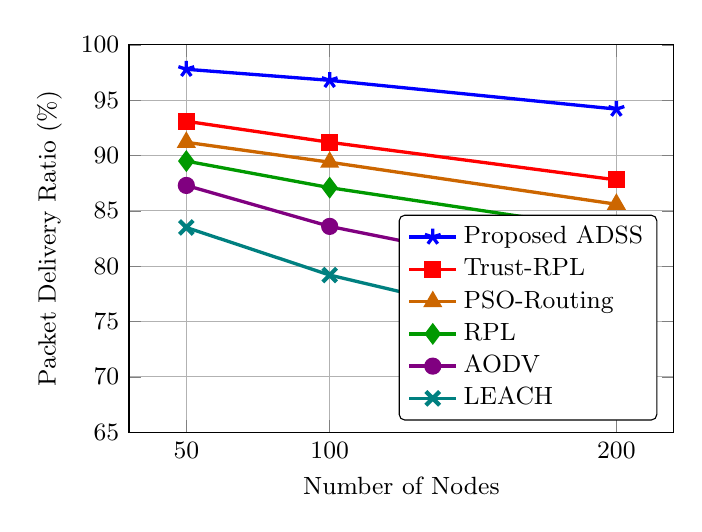
\begin{tikzpicture}
\begin{axis}[
    width=8.5cm,
    height=6.5cm,
    xlabel={Number of Nodes},
    ylabel={Packet Delivery Ratio (\%)},
    xmin=30, xmax=220,
    ymin=65, ymax=100,
    xtick={50,100,200},
    xticklabels={50,100,200},
    ytick={65,70,75,80,85,90,95,100},
    grid=both,
    grid style={line width=0.2pt, draw=gray!30},
    major grid style={line width=0.4pt, draw=gray!60},
    legend style={
        at={(0.97,0.03)},
        anchor=south east,
        font=\small,
        cells={anchor=west},
        fill=white,
        draw=black,
        rounded corners=2pt,
    },
    tick label style={font=\small},
    label style={font=\small},
    title style={font=\small\bfseries},
    every axis plot/.append style={line width=1.2pt},
]
% Proposed ADSS
\addplot[color=blue, mark=star, mark size=3pt]
    coordinates {(50,97.8) (100,96.8) (200,94.2)};
\addlegendentry{Proposed ADSS}
% Trust-RPL
\addplot[color=red, mark=square*, mark size=2.5pt]
    coordinates {(50,93.1) (100,91.2) (200,87.8)};
\addlegendentry{Trust-RPL}
% PSO-Routing
\addplot[color=orange!80!black, mark=triangle*, mark size=2.8pt]
    coordinates {(50,91.2) (100,89.4) (200,85.6)};
\addlegendentry{PSO-Routing}
% RPL
\addplot[color=green!60!black, mark=diamond*, mark size=3pt]
    coordinates {(50,89.5) (100,87.1) (200,83.2)};
\addlegendentry{RPL}
% AODV
\addplot[color=violet, mark=*, mark size=2.5pt]
    coordinates {(50,87.3) (100,83.6) (200,78.4)};
\addlegendentry{AODV}
% LEACH
\addplot[color=teal, mark=x, mark size=3.5pt, mark options={line width=1.5pt}]
    coordinates {(50,83.5) (100,79.2) (200,73.1)};
\addlegendentry{LEACH}
\end{axis}
\end{tikzpicture}
\end{document}

\documentclass[tikz,border=4pt]{standalone}
\usepackage{pgfplots}
\pgfplotsset{compat=1.18}

\begin{document}
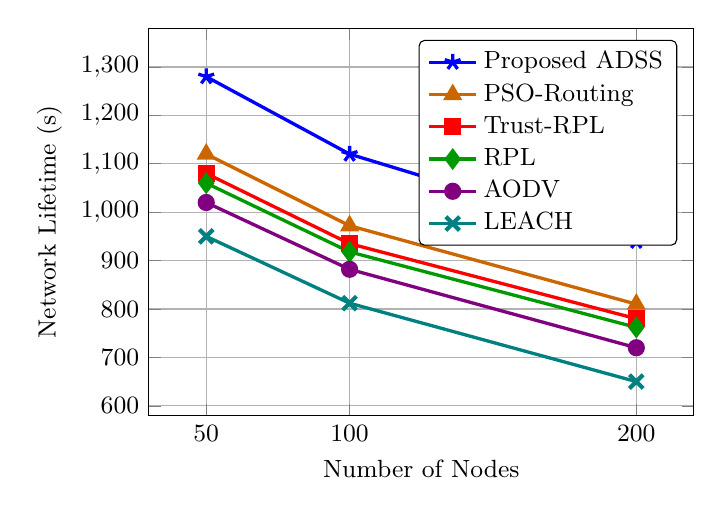
\begin{tikzpicture}
\begin{axis}[
    width=8.5cm,
    height=6.5cm,
    xlabel={Number of Nodes},
    ylabel={Network Lifetime (s)},
    xmin=30, xmax=220,
    ymin=580, ymax=1380,
    xtick={50,100,200},
    xticklabels={50,100,200},
    ytick={600,700,800,900,1000,1100,1200,1300},
    grid=both,
    grid style={line width=0.2pt, draw=gray!30},
    major grid style={line width=0.4pt, draw=gray!60},
    legend style={
        at={(0.97,0.97)},
        anchor=north east,
        font=\small,
        cells={anchor=west},
        fill=white,
        draw=black,
        rounded corners=2pt,
    },
    tick label style={font=\small},
    label style={font=\small},
    every axis plot/.append style={line width=1.2pt},
]
% Proposed ADSS
\addplot[color=blue, mark=star, mark size=3pt]
    coordinates {(50,1280) (100,1120) (200,940)};
\addlegendentry{Proposed ADSS}
% PSO-Routing
\addplot[color=orange!80!black, mark=triangle*, mark size=2.8pt]
    coordinates {(50,1120) (100,972) (200,810)};
\addlegendentry{PSO-Routing}
% Trust-RPL
\addplot[color=red, mark=square*, mark size=2.5pt]
    coordinates {(50,1080) (100,935) (200,780)};
\addlegendentry{Trust-RPL}
% RPL
\addplot[color=green!60!black, mark=diamond*, mark size=3pt]
    coordinates {(50,1060) (100,918) (200,762)};
\addlegendentry{RPL}
% AODV
\addplot[color=violet, mark=*, mark size=2.5pt]
    coordinates {(50,1020) (100,882) (200,720)};
\addlegendentry{AODV}
% LEACH
\addplot[color=teal, mark=x, mark size=3.5pt, mark options={line width=1.5pt}]
    coordinates {(50,950) (100,812) (200,650)};
\addlegendentry{LEACH}
\end{axis}
\end{tikzpicture}
\end{document}

\documentclass[tikz,border=4pt]{standalone}
\usepackage{pgfplots}
\pgfplotsset{compat=1.18}

\begin{document}
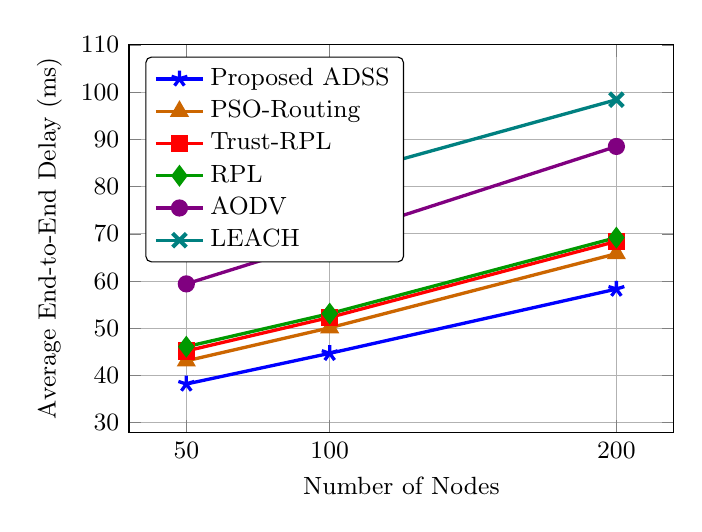
\begin{tikzpicture}
\begin{axis}[
    width=8.5cm,
    height=6.5cm,
    xlabel={Number of Nodes},
    ylabel={Average End-to-End Delay (ms)},
    xmin=30, xmax=220,
    ymin=28, ymax=110,
    xtick={50,100,200},
    xticklabels={50,100,200},
    ytick={30,40,50,60,70,80,90,100,110},
    grid=both,
    grid style={line width=0.2pt, draw=gray!30},
    major grid style={line width=0.4pt, draw=gray!60},
    legend style={
        at={(0.03,0.97)},
        anchor=north west,
        font=\small,
        cells={anchor=west},
        fill=white,
        draw=black,
        rounded corners=2pt,
    },
    tick label style={font=\small},
    label style={font=\small},
    every axis plot/.append style={line width=1.2pt},
]
% Proposed ADSS
\addplot[color=blue, mark=star, mark size=3pt]
    coordinates {(50,38.2) (100,44.7) (200,58.3)};
\addlegendentry{Proposed ADSS}
% PSO-Routing
\addplot[color=orange!80!black, mark=triangle*, mark size=2.8pt]
    coordinates {(50,43.1) (100,50.1) (200,65.8)};
\addlegendentry{PSO-Routing}
% Trust-RPL
\addplot[color=red, mark=square*, mark size=2.5pt]
    coordinates {(50,45.2) (100,52.3) (200,68.4)};
\addlegendentry{Trust-RPL}
% RPL
\addplot[color=green!60!black, mark=diamond*, mark size=3pt]
    coordinates {(50,46.1) (100,53.1) (200,69.2)};
\addlegendentry{RPL}
% AODV
\addplot[color=violet, mark=*, mark size=2.5pt]
    coordinates {(50,59.4) (100,68.9) (200,88.5)};
\addlegendentry{AODV}
% LEACH
\addplot[color=teal, mark=x, mark size=3.5pt, mark options={line width=1.5pt}]
    coordinates {(50,70.2) (100,81.6) (200,98.4)};
\addlegendentry{LEACH}
\end{axis}
\end{tikzpicture}
\end{document}

\documentclass[tikz,border=4pt]{standalone}
\usepackage{pgfplots}
\pgfplotsset{compat=1.18}

\begin{document}
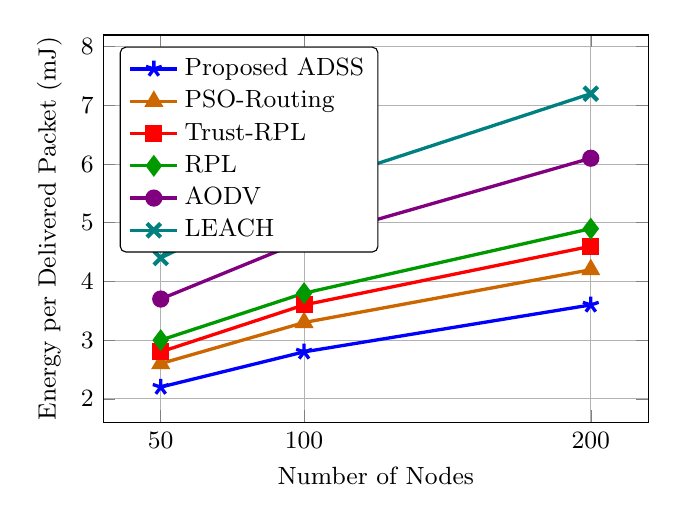
\begin{tikzpicture}
\begin{axis}[
    width=8.5cm,
    height=6.5cm,
    xlabel={Number of Nodes},
    ylabel={Energy per Delivered Packet (mJ)},
    xmin=30, xmax=220,
    ymin=1.6, ymax=8.2,
    xtick={50,100,200},
    xticklabels={50,100,200},
    ytick={2,3,4,5,6,7,8},
    grid=both,
    grid style={line width=0.2pt, draw=gray!30},
    major grid style={line width=0.4pt, draw=gray!60},
    legend style={
        at={(0.03,0.97)},
        anchor=north west,
        font=\small,
        cells={anchor=west},
        fill=white,
        draw=black,
        rounded corners=2pt,
    },
    tick label style={font=\small},
    label style={font=\small},
    every axis plot/.append style={line width=1.2pt},
]
% Proposed ADSS
\addplot[color=blue, mark=star, mark size=3pt]
    coordinates {(50,2.2) (100,2.8) (200,3.6)};
\addlegendentry{Proposed ADSS}
% PSO-Routing
\addplot[color=orange!80!black, mark=triangle*, mark size=2.8pt]
    coordinates {(50,2.6) (100,3.3) (200,4.2)};
\addlegendentry{PSO-Routing}
% Trust-RPL
\addplot[color=red, mark=square*, mark size=2.5pt]
    coordinates {(50,2.8) (100,3.6) (200,4.6)};
\addlegendentry{Trust-RPL}
% RPL
\addplot[color=green!60!black, mark=diamond*, mark size=3pt]
    coordinates {(50,3.0) (100,3.8) (200,4.9)};
\addlegendentry{RPL}
% AODV
\addplot[color=violet, mark=*, mark size=2.5pt]
    coordinates {(50,3.7) (100,4.7) (200,6.1)};
\addlegendentry{AODV}
% LEACH
\addplot[color=teal, mark=x, mark size=3.5pt, mark options={line width=1.5pt}]
    coordinates {(50,4.4) (100,5.6) (200,7.2)};
\addlegendentry{LEACH}
\end{axis}
\end{tikzpicture}
\end{document}
